\documentclass{article}
\usepackage[french]{babel}
\usepackage[T1]{fontenc}
\usepackage[autolanguage,np]{numprint} % tableau spécial
\usepackage[left=2cm,right=2cm,top=2cm,bottom=2cm]{geometry}
\usepackage{fancyhdr}
\pagestyle{fancy}
\chead{Boucliers}
\usepackage{multicol}

\usepackage{fontspec}
\defaultfontfeatures{Ligatures=TeX}
%\setmainfont[Mapping=tex-text]{Sitka Display}
\usepackage[small,sf,bf]{titlesec}

\usepackage{graphicx}
\usepackage{xcolor}
\usepackage{colortbl} % table color
\usepackage{tabularray}
\usepackage{makecell}
\usepackage{sectsty}
\usepackage{wasysym} % \male and \female icons

% Color definition
\definecolor{DarkGreen}{HTML}{384d3e}
\definecolor{PureWhite}{HTML}{FFFFFF}
\definecolor{DarkRed}{HTML}{6e272d}
\definecolor{DarkGold}{HTML}{a48e3b}

% Each part and section has its own color
\partfont{\color{DarkGreen}}
\sectionfont{\color{DarkRed}}
\subsectionfont{\color{DarkGold}}
\subsubsectionfont{\color{DarkRed}}

% Variable definition
%% Special table horizontal space for first column
\newcommand{\specialtablehspace}{0.5cm}

%% Dices
\newcommand{\diceblack}{\hspace{0.1cm}{\Large
\includegraphics[height=\fontcharht\font`\B]{../_img/dice_black}}\hspace{0.1cm}}
\newcommand{\diceblue}{\hspace{0.1cm}{\Large 
\includegraphics[height=\fontcharht\font`\B]{../_img/dice_blue}}\hspace{0.1cm}}
\newcommand{\dicegreen}{\hspace{0.1cm}{\Large 
\includegraphics[height=\fontcharht\font`\B]{../_img/dice_green}}\hspace{0.1cm}}
\newcommand{\dicepurple}{\hspace{0.1cm}{\Large 
\includegraphics[height=\fontcharht\font`\B]{../_img/dice_purple}}\hspace{0.1cm}}
\newcommand{\dicered}{\hspace{0.1cm}{\Large 
\includegraphics[height=\fontcharht\font`\B]{../_img/dice_red}}\hspace{0.1cm}}
\newcommand{\diceyellow}{\hspace{0.1cm}{\Large 
\includegraphics[height=\fontcharht\font`\B]{../_img/dice_yellow}}\hspace{0.1cm}}
\newcommand{\diceadvantage}{\hspace{0.1cm}{\Large 
\includegraphics[height=\fontcharht\font`\B]{../_img/result_avantage_advantage}}\hspace{0.1cm}}
\newcommand{\dicedespair}{\hspace{0.1cm}{\Large 
\includegraphics[height=\fontcharht\font`\B]{../_img/result_desastre_despair}}\hspace{0.1cm}}
\newcommand{\dicefailure}{\hspace{0.1cm}{\Large 
\includegraphics[height=\fontcharht\font`\B]{../_img/result_echec_failure}}\hspace{0.1cm}}
\newcommand{\dicethreat}{\hspace{0.1cm}{\Large 
\includegraphics[height=\fontcharht\font`\B]{../_img/result_menace_threat}}\hspace{0.1cm}}
\newcommand{\dicesuccess}{\hspace{0.1cm}{\Large 
\includegraphics[height=\fontcharht\font`\B]{../_img/result_succes_success}}\hspace{0.1cm}}
\newcommand{\dicetriumph}{\hspace{0.1cm}{\Large 
\includegraphics[height=\fontcharht\font`\B]{../_img/result_triomphe_triumph}}\hspace{0.1cm}}

\author{}

\begin{document}

\title{\vspace{-0.5cm}{\Huge Boucliers} \vspace{-1cm}}

\date{}

\maketitle

% One page title
% \vspace{4cm}
% Pariatur voluptate in non ex adipisicing ut et duis Lorem elit laborum. Ullamco cupidatat est magna nostrud velit duis ipsum do consequat cillum in labore aute. Anim ipsum officia quis et amet do proident voluptate voluptate qui.
% \clearpage

% table of content
% \tableofcontents
% \clearpage

\part*{Introduction}
Dans le système Star Wars FFG, les petits véhicules souffrent souvent d’un manque de résistance face aux assauts répétés. Cette règle maison propose une alternative : remplacer les dés \diceblack actuels par une mécanique plus représentative de l’efficacité de leurs boucliers. Chaque point de bouclier confère un dé \diceblack supplémentaire. Ce dé peut ajouter soit un \dicefailure, soit un \dicethreat (avantage), ou une combinaison des deux, au jet d’attaque ennemi.

\paragraph{}
Ainsi, les petits appareils bénéficient d’une protection plus tangible, même si cela reste une défense partielle. Toutefois, cette adaptation ne reflète pas entièrement le fonctionnement des boucliers déflecteurs, qui, eux, sont conçus pour annuler purement et simplement les dégâts.


\begin{figure}[!h]
    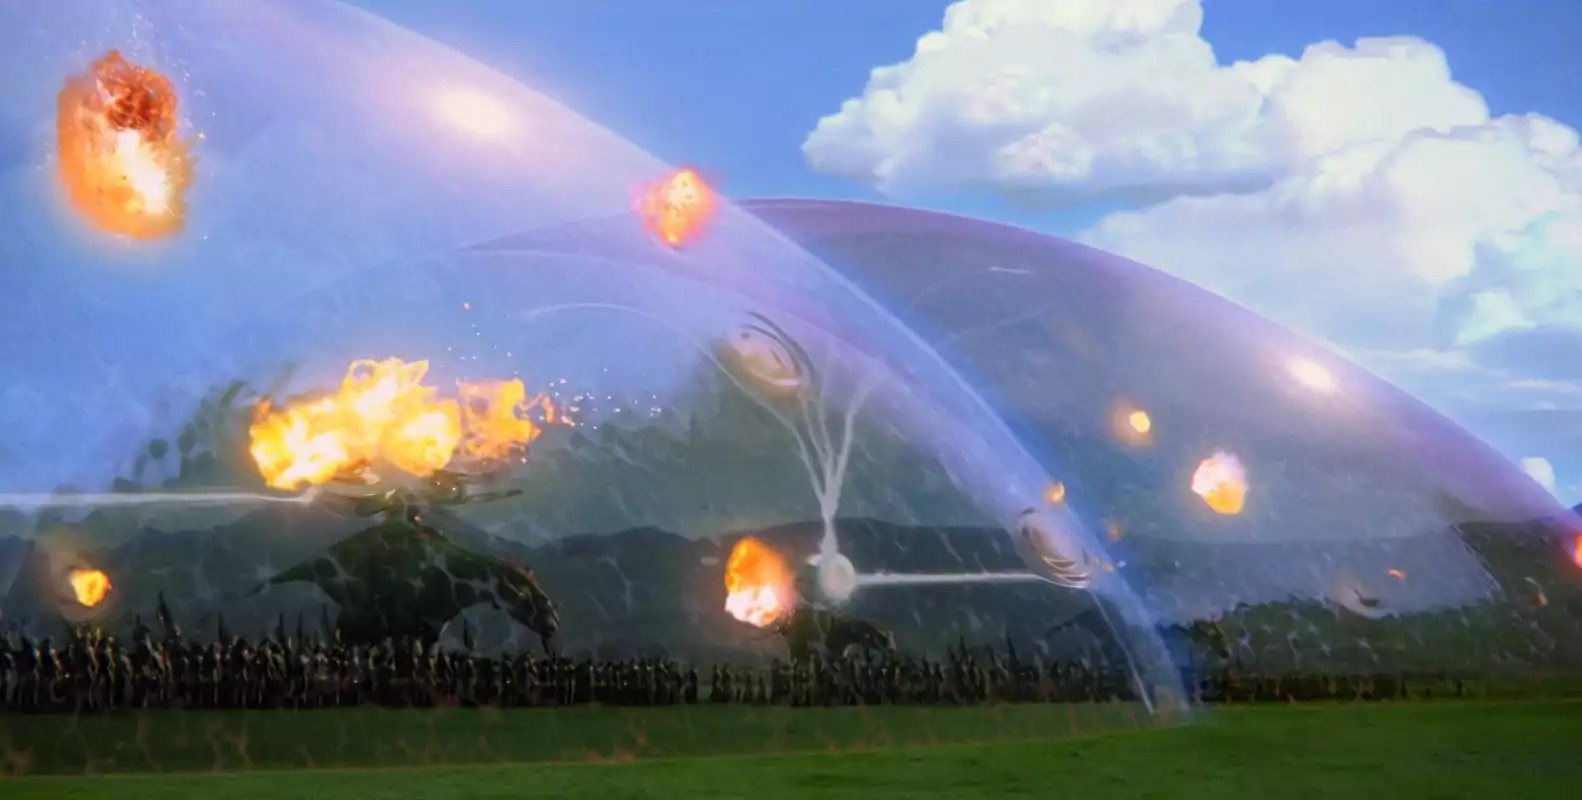
\includegraphics[width=1\linewidth]{../_img/boucliers/bouclier.jpg}
	\caption{Exemple de bouclier}
\end{figure}
%Par exemple
%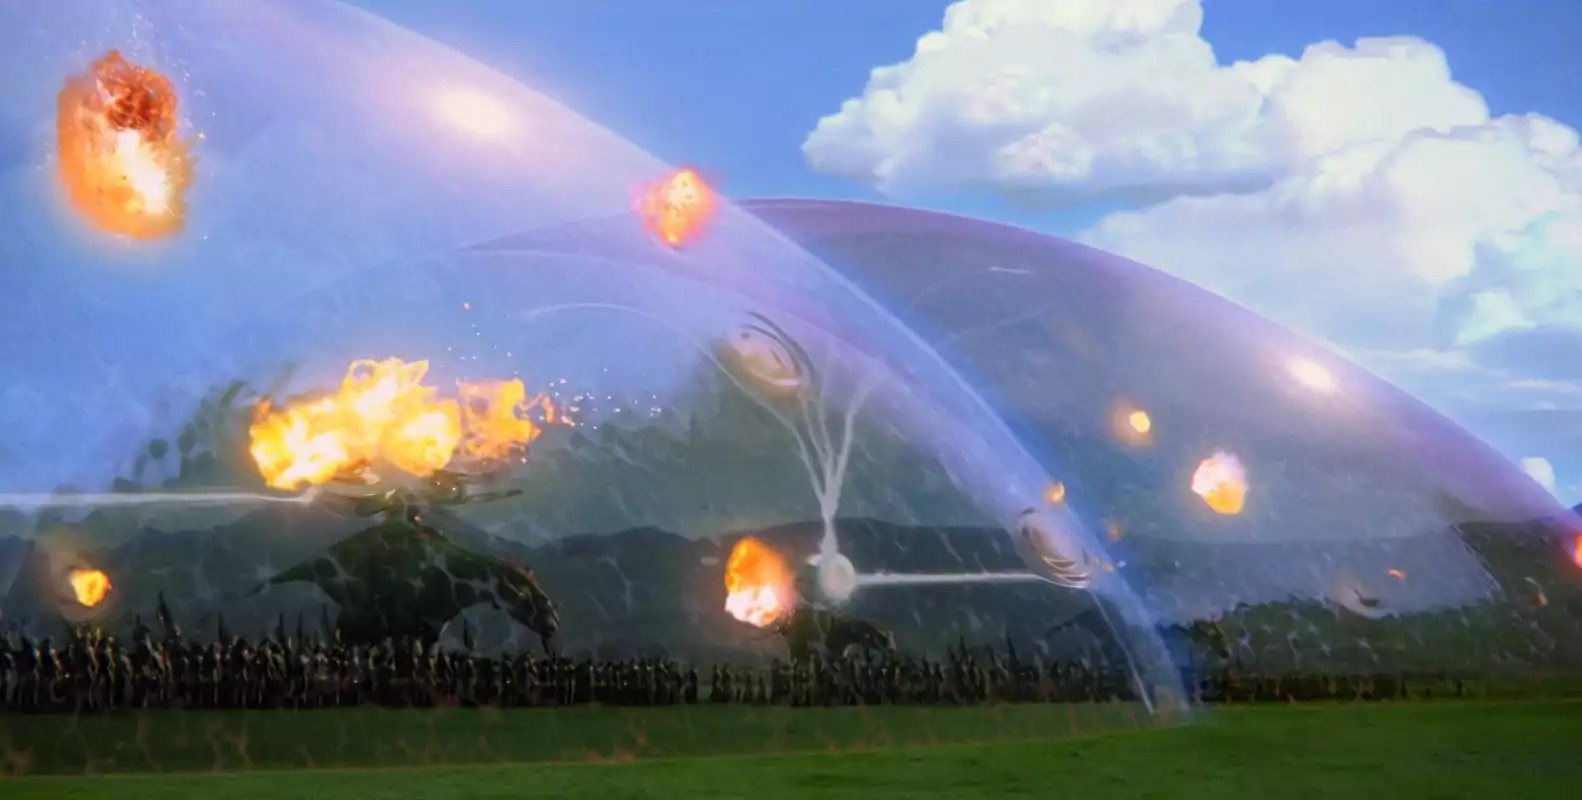
\includegraphics[width=1\linewidth]{../_img/boucliers/bouclier.jpg}

Les obus, les tirs de blaster et autres projectiles frappent le bouclier et explosent à sa surface, forçant l’armée droïde à devoir franchir la barrière d’énergie avant de pouvoir tirer sur les Gungans. C’est ce que l’on voit dans les films, et c’est exactement ce que j’aimerais retrouver en jeu, pour que les joueurs puissent visualiser ce fonctionnement immédiatement.

Mais dans le système actuel, les personnages dépensent généralement tout leur argent dans des réparations de blindage de coque, car les boucliers basés sur les dés \diceblack n’arrêtent pratiquement aucun dégât significatif. En moyenne, ils ne servent qu’environ deux fois sur trois… ce qui est loin d’être suffisant. Sur les chasseurs stellaires — déjà de véritables cercueils volants — cela veut dire qu’on finit vite transformé en toast spatial.

\paragraph{}
Première étape : mettez de côté les dés \diceblack, on n’en a plus besoin.
À la place, utilisons une mécanique bien plus simple, purement numérique : chaque vaisseau avec un bouclier dispose généralement de 1 ou 2 points de protection sur une zone, les plus gros peuvent monter à 3 ou 4, et certains Talents de pilote (par exemple Conduite défensive) peuvent encore en rajouter 1 ou 2. Nous allons conserver un plafond de 4 points maximum par moyens techniques, plus les éventuels bonus de Talents.

\paragraph{}
Ce score de Bouclier reste une valeur numérique, inchangée pour éviter toute confusion, et continue de s’appliquer aux mécaniques déjà présentes du système (comme les collisions ou les impacts environnementaux). La seule différence : on transforme cette Valeur de Bouclier en nombre de coups absorbés. Bien entendu, les boucliers existent sous différentes formes et tailles, variant selon le type de vaisseau qui les porte. Les petits appareils n’ont pas assez de puissance pour alimenter un générateur digne d’une frégate, et inversement un modèle conçu pour un cargo ne couvrira jamais un croiseur. Mais tous ces boucliers partagent un point commun : ils protègent une arc de tir spécifique.

\paragraph{}
\begin{tabular}{|c|c|c|}
	\hline 
	\cellcolor{DarkRed} {\textcolor{PureWhite}{\textbf{Gabarit}}} & \cellcolor{DarkRed} {\textcolor{PureWhite}{\textbf{Valeur de bouclier}}} \\ 
	\hline 
	2 -- 3 & 6 coups par arc \\ 
	\hline 
	4 -- 5 & 10 coups par arc \\ 
	\hline 
	6 -- 7 & 10 + Gabarit par arc \\ 
	\hline 
	8 -- 9 & 12 + Gabarit par arc \\ 
	\hline 
	2 -- 3 & 15 + Gabarit par arc \\ 
	\hline 
\end{tabular}


\section*{Exemple d’application de la règle maison}
X-Wing
\begin{itemize}
	\item Boucliers : 1 Avant, 1 Arrière
	\item Chaque point de Bouclier correspond à 6 Coups absorbés dans l’arc qu’il protège.
	\item Résultat : 6 Coups absorbés à l’Avant et 6 Coups absorbés à l’Arrière.
\end{itemize}

Frégate Nebulon-B
\begin{itemize}
	\item Boucliers : 2 / 2 / 2 / 2 (sur ses quatre arcs)
	\item Calcul : (10 + 6) × 2 = 32 Coups absorbés par arc défensif.
\end{itemize}

\paragraph{}
La logique est simple : 1 point de Bouclier = 6 coups absorbés. Certains vaisseaux plus massifs (comme la Nebulon-B) utilisent une formule étendue : (10 + 6) multiplié par le nombre de boucliers sur l’arc.


\part*{Les Mécaniques des Boucliers}

\begin{quote}
\textit{« Monsieur, nous venons de perdre le bouclier déflecteur arrière principal ! 
Un coup direct de plus sur le quart arrière et nous sommes finis ! »} \\
--- C-3PO
\end{quote}

Être pourchassé dans l’espace par un \textbf{Destroyer Stellaire} est rarement une activité reposante\dots sauf si l’on bénéficie de \textbf{10 mètres d’armure scénaristique}, comme dans les films. Ces règles ne rendront pas vos vaisseaux invincibles, mais elles éviteront peut-être que le moindre escadron de TIE  transforme votre \textbf{YT-1300} en ferraille volante.

\section*{Règle de base : gestion des dégâts}
\begin{itemize}
  \item Tout dégât \textbf{frappe d’abord les boucliers}.
  \item Appliquez ensuite normalement l’\textbf{armure du vaisseau (soak)}.
\end{itemize}

\paragraph{Exemple :}
Un TIE tire sur un \textbf{YT-1300} dont l’arc arrière est protégé par \textbf{1 Bouclier (10 points)} :
\begin{itemize}
  \item Le TIE inflige \textbf{9 dégâts}.
  \item Le YT-1300 a une \textbf{Armure de 3} $\rightarrow$ $9 - 3 = 6$ points de dégâts absorbés par le bouclier arrière.
  \item Le bouclier arrière tombe donc à \textbf{4 points restants}.
\end{itemize}

Si le pilote TIE déclenche ses \textbf{canons jumelés} (2 × 9 dégâts) :
\begin{itemize}
  \item Première salve : le bouclier tombe à 4.
  \item Seconde salve : $9 - 3 = 6$ dégâts, dont 4 absorbés par le bouclier, et 2 passent en \textbf{Traumatismes de coque}.
  \item Le \textbf{bouclier arrière est détruit}.
\end{itemize}

\begin{itemize}
  \item \textbf{Brêche} fonctionne normalement avec les armes puissantes.
  \item \textbf{Réorienter les boucliers déflecteurs} reste une manœuvre standard d’équipage.
\end{itemize}

\section*{Le rôle de l’Ingénieur}

L’ingénieur n’est plus un simple figurant : les boucliers lui donnent une vraie place !

\paragraph{Booster les boucliers :}
\begin{itemize}
  \item Test de \textbf{Mécanique Difficile (\dicepurple\dicepurple\dicepurple)}.
  \item En cas de succès : augmente la \textbf{Zone de défense} de +1 jusqu’au début du prochain tour.
  \item Chaque \dicesuccess supplémentaire prolonge l’effet d’un round.
  \item Exemple : un \textbf{YT-1300} avec 10 points sur son bouclier arrière passe temporairement à \textbf{20 points}.
\end{itemize}

\paragraph{Réparer les boucliers (nouvelle action maison) :}
\begin{itemize}
  \item Test de \textbf{Mécanique Difficile (\dicepurple\dicepurple\dicepurple)}.
  \item Permet de restaurer un arc déflecteur tombé à zéro.
  \item Coût : \textbf{2 × le Seuil de Stress Mécanique}.
  \item Chaque \diceadvantage réduit le coût, minimum 1.
  \item Un bouclier détruit par un \textbf{Coup Critique} ne peut pas être restauré.
\end{itemize}

\section*{Le rôle du Pilote}

Les pilotes disposant du talent \textbf{Conduite défensive} deviennent cruciaux.

\begin{itemize}
  \item Chaque rang ajoute une \textbf{réserve temporaire de 10 points par arc déflecteur}.
  \item Ces points s’utilisent avant les boucliers mécaniques.
  \item Ils se régénèrent à chaque action du pilote.
\end{itemize}

\paragraph{Exemple :}
\textit{Bob le contrebandier} a 1 rang de \textbf{Conduite défensive} dans son YT-1300 :
\begin{itemize}
  \item Chaque arc bénéficie de \textbf{10 points temporaires}.
  \item Ils absorbent les premiers dégâts avant les boucliers.
  \item Au tour suivant de Bob, cette réserve se recharge automatiquement.
\end{itemize}

\section*{Conclusion}
Ce système rend les vaisseaux \textbf{plus résistants}.  
Si vous trouvez vos parties trop « blindées », ajustez les valeurs.  
Mais il corrige surtout la \textbf{fragilité extrême des chasseurs} et évite l’effet \textit{Rocket Tag}, 
où l’initiative seule décide du combat.  

\bigskip
\textbf{Cette règle maison est gratuite et libre d’utilisation.}  
Utilisez-la pour donner plus de souffle (et de survie !) à vos combats spatiaux.

\end{document}
